\documentclass[10pt,conference,compsocconf]{IEEEtran}

\usepackage{hyperref}
\usepackage{graphicx}	% For figure environment


\begin{document}
\title{Digital 3D Geometry Processing - Project\\
Deliverable 1}

\author{
  Rapha\"{e}l Steinmann\\
	Thomas Batschelet\\
	Alain Milliet\\
  \textit{Department of Computer Science, EPFL, Switzerland}
}

\maketitle


\section{Goals}
\label{sec:goals}
We would like to create a lamp mesh that is visually aesthetic, gives interesting lightning effects and is challenging from an implementation point of view. Therefore, after some thinking and research we agreed on the concept of a "water-like mesh". It means we would have to simulate a liquid trickling down the mesh while partially reproducing its shape (see Figure~\ref{fig:water}).

The implementation seems very challenging, hence we prefer to have a plan B in case it turns out to be unfeasible without using a software. Plan B would be to apply some artistic pattern on the mesh and disable some faces in order to create holes in it. (Like in the example~\ref{fig:bear})

For both of this implementation we will need to have a really clean and smooth model at the beginning. See section ~\ref{sec:tools} for more details on what tools we will use to clean our mesh.


\section{Methods}
\label{sec:methods}
To reach our goals we will need to implement several methods. First of all we will have to smooth our mesh and make it as uniform as possible (vertex/face/edge-wise). For this matter we will use techniques we have seen during the course and labs (using curvature to smooth the object for example).\\
We will also need to come up with our own new methods if we want to achieve a result that looks like Figure~\ref{fig:water}. We need to implement methods that use fluid dynamics and constraints.

\section{Tools}
\label{sec:tools}
For this project we will use different existing tools to clean our mesh. We will first of all use Meshlab to remove several default our mesh can contain (duplicate faces and vertices, zero area faces, unreferenced vertices and other possible problems). We will also use Meshlab to reduce the number of triangles contained in the mesh. (At the moment the number is really high)\\\\
Then we will use Netfabb to make a default repair of the mesh. The repair should fix the following problems if necessary: 
\begin{enumerate}
\item Zero Holes: model will be manifold, without any gaps between faces and edges.
\item Zero Border Edges: a border edge is an edge on the side of a hole, or the edge side of a plane if another edge is missing.
\item Zero Invalid Orientations: In Netfabb, the direction of a face is shown in green if it points outward, red if it points inward. If you have red faces pointing out, that will be invalid orientation because it is inconsistent.
\item Positive Volume: All the green faces face outside and the red faces inside, otherwise the printer will think that everything outside the model is material causing printer issues.
\item Closed Surfaces: A closed surface means that there are no holes or border edges.
\item Orientable Surface: Each face must be defined as in or out, with no stray edges or vertices.
\end{enumerate}

\begin{figure}[tbp]
	\centering
	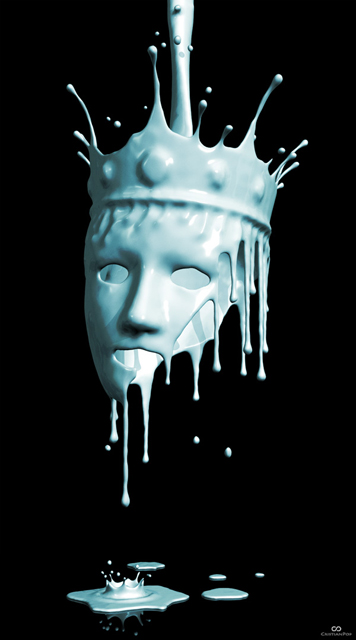
\includegraphics[width=\columnwidth]{liquid_mesh}
	\caption{Simulate water falling down a mesh}
	\vspace{-3mm}
	\label{fig:water}
\end{figure}

\begin{figure}[tbp]
	\centering
	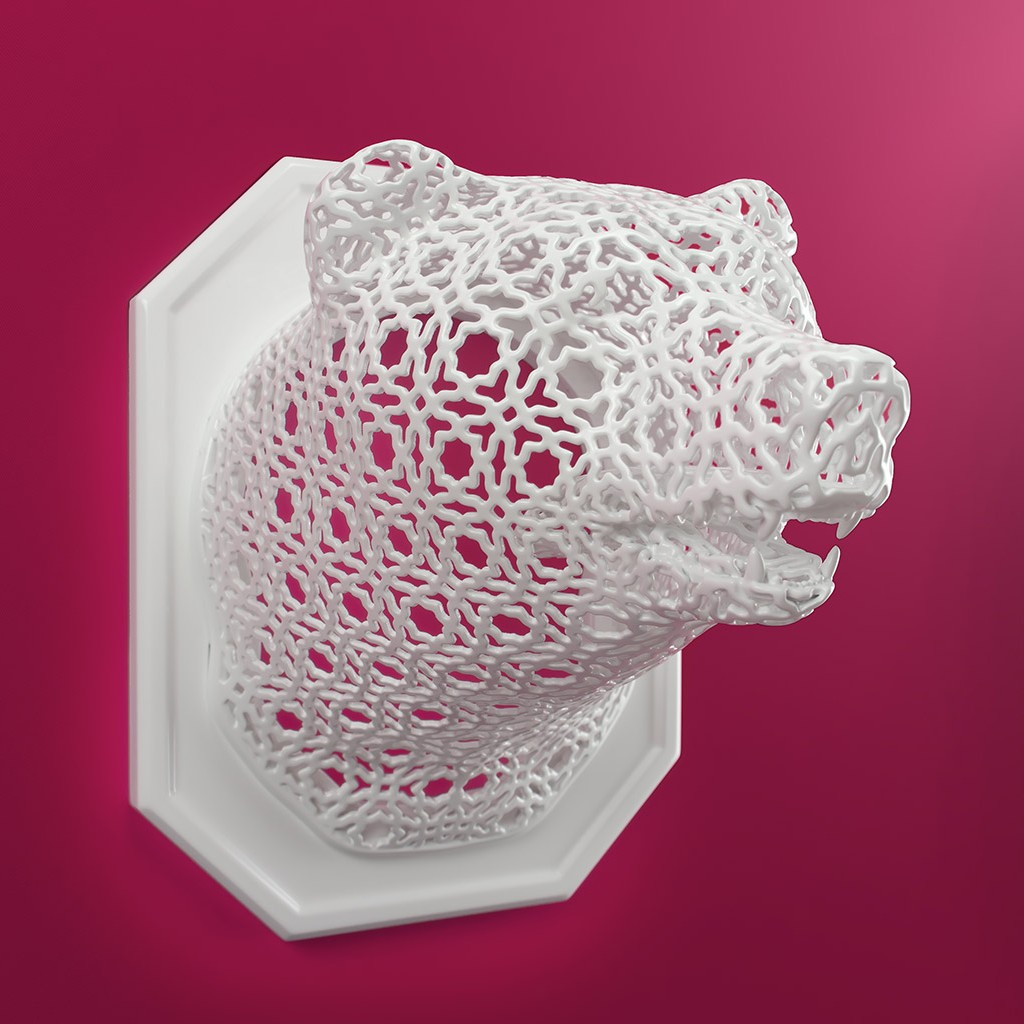
\includegraphics[width=\columnwidth]{3d-printed-lamps-animal-lace-bear}
	\caption{Pattern application on a bear-like mesh (taken from the examples in the project description)}
	\vspace{-3mm}
	\label{fig:bear}
\end{figure}

\end{document}
